
\newcommand{\CC}{\cellcolor{Gray}}
\definecolor{Gray}{gray}{0.9}

\subsection{Experimental Evaluation of UDS}
\label{sec:exp}
In our experiments, we aim to evaluate whether the theoretical potential for simple minimum-reward relabeling to attain good results is reflected in benchmark tasks and more complex offline RL settings. In particular, we will study: \textbf{(1)} can UDS match or exceed the performance of sophisticated reward inference methods and methods with oracle reward functions in simulated locomotion and navigation tasks? \textbf{(2)} can combining with CDS further improve the results achieved by UDS?, \textbf{(3)} how does UDS behave with and without combining with an optimized reweighting strategy in multi-task offline RL settings?, \textbf{(4)} under which conditions does UDS work and not work and does optimizing for reweighting via CDS help?

\begin{table*}[ht]
% \vspace{-0.2cm}
\caption{\footnotesize Results for multi-task robotic manipulation (Meta-World) and navigation environments (AntMaze) with low-dimensional state inputs. Numbers are averaged across 6 seeds, $\pm$ the 95$\%$-confidence interval. We take the results of No Sharing, Sharing All and CDS, directly from \cite{yu2021conservative}. We bold the best-performing method that does not have access to the true rewards for relabeling. We include per-task performance for Meta-World domains and the overall performance averaged across tasks (highlighted in gray) for all three domains. Both CDS+UDS and UDS outperforms prior vanilla multi-task offline RL approach (No Sharing) and reward learning methods (Reward Predictor, VICE and RCE) while performing competitively compared to oracle reward relabeling methods.}
\vspace{-0.4cm}
\begin{center}
\resizebox{\textwidth}{!}{\begin{tabular}{l|l|rrrrrr|rr}
\toprule
& & & & & & & & \multicolumn{2}{c}{\textbf{Oracle Methods}} \\
\textbf{Environment} & \textbf{Tasks} & \textbf{CDS+UDS} & \textbf{UDS} & \textbf{VICE} & \textbf{RCE} & \textbf{No Sharing} & \textbf{Reward Pred.} & \textbf{CDS} & \textbf{Sharing All}\\ \midrule
& door open & \textbf{61.3\%}$\pm$7.9\% & 51.9\%$\pm$25.3\% & 0.0\%$\pm$0.0\% & 0.0\%$\pm$0.0\% & 14.5\%$\pm$12.7\% & 0.0\%$\pm$0.0\% & 58.4\%$\pm$9.3\% & 34.3\%$\pm$17.9\%\\
& door close & 54.0\% $\pm$42.5\% & 12.3\%$\pm$27.6\% & 66.7\%\%$\pm$47.1\% & 0.0\%$\pm$0.0\% & 4.0\%$\pm$6.1\% & \textbf{99.3\%}$\pm$0.9\% & 65.3\%$\pm$27.7\% & 48.3\%$\pm$27.3\%\\
Meta-World& drawer open & \textbf{73.5\%}$\pm$9.6\% & 61.8\%$\pm$16.3\% & 0.0\%$\pm$0.0\% & 0.0\%$\pm$0.0\% & 16.0\%$\pm$17.5\% & 13.3\%$\pm$18.9\% & 57.9\%$\pm$16.2\% & 55.1\%$\pm$9.4\%\\
& drawer close & 99.3\%$\pm$0.7\% & \textbf{99.6\%}$\pm$0.7\% & 19.3\%$\pm$27.3\% & 2.7\%$\pm$1.7\% & 99.0\%$\pm$0.7\% & 50.3\%$\pm$35.8\% & 99.0\%$\pm$0.7\% & 98.8\%$\pm$0.7\%\\
& \CC \textbf{average} & \CC \textbf{71.2\%} $\pm$ 11.3\% & \CC 56.4\%$\pm$12.8\% & \CC 21.5\%$\pm$0.7\% & \CC 0.7\%$\pm$0.4\% & \CC 33.4\%$\pm$8.3\% & \CC 41.0\%$\pm$11.9\% & \CC 70.1\%$\pm$8.1\% & \CC 59.4\%$\pm$5.7\%\\
\midrule
AntMaze    & medium (3 tasks)  &\textbf{31.5\%}$\pm$3.0\% & 26.5\%$\pm$9.1\%  & 2.9\%$\pm$1.0\%  & 0.0\%$\pm$0.0\%  & 21.6\%$\pm$7.1\% & 3.8\%$\pm$3.8\% & 36.7\%$\pm$6.2\%  & 22.9\%$\pm$3.6\%\\
& large (7 tasks)  & \textbf{18.4\%}$\pm$6.1\% & 14.2\%$\pm$3.9\% & 2.5\%$\pm$1.1\% & 0.0\%$\pm$0.0\% & 13.3\% $\pm$ 8.6\% & 5.9\%$\pm$4.1\% & 22.8\% $\pm$ 4.5\% & 16.7\% $\pm$ 7.0\%\\
\bottomrule
\end{tabular}}
\end{center}
\vspace{-0.3cm}
\label{tbl:gym}
\normalsize
\end{table*}


\begin{table*}[ht]
\vspace*{-0.3cm}
\caption{\footnotesize Results for multi-task imaged-based robotic manipulation domains in \citep{yu2021conservative}. Numbers are averaged across 3 seeds, $\pm$ the 95$\%$ confidence interval. UDS outperforms No Sharing in 7 out of 10 tasks as well as the average task performance, while performing comparably to Sharing All. CDS+UDS further improves the performance of UDS and outperforms No Sharing in all of the 10 tasks.
}
\vspace{-0.3cm}
\small{
\begin{center}
\resizebox{0.99\textwidth}{!}{\begin{tabular}{l|rrr|rr}
\toprule
\textbf{Task Name} & \textbf{CDS+UDS}& \textbf{UDS} & \textbf{No Sharing} & \textbf{CDS (oracle)} & \textbf{Sharing All (oracle)}\\ \midrule
\texttt{lift-banana} & \textbf{55.9\%}$\pm$11.7\% & 48.6\%$\pm$5.1\% & 20.0\%$\pm$6.0\% &  \textbf{53.1\%}$\pm$3.2\% & 41.8\%$\pm$4.2\%\\
\texttt{lift-bottle} & \textbf{72.9\%}$\pm$12.8\% & 58.1\%$\pm$3.6\%& 49.7\%$\pm$8.7\% & \textbf{74.0\%}$\pm$6.3\% & 60.1\%$\pm$10.2\%\\
\texttt{lift-sausage} & \textbf{74.3\%}$\pm$8.3\%  & 66.8\% $\pm$ 2.7\%  & 60.9\%$\pm$6.6\% & \textbf{71.8\%}$\pm$3.9\% & 70.0\%$\pm$7.0\%\\
\texttt{lift-milk}& 73.5\%$\pm$6.7\% & \textbf{74.5\%}$\pm$2.5\% & 68.4\%$\pm$6.1\% & \textbf{83.4\%}$\pm$5.2\% & 72.5\%$\pm$5.3\%\\

\texttt{lift-food} & \textbf{66.3\%}$\pm$8.3\% & 53.8\%$\pm$8.8\%  & 39.1\%$\pm$7.0\% & \textbf{61.4\%}$\pm$9.5\% & 58.5\%$\pm$7.0\%\\
\texttt{lift-can} & \textbf{64.9\%}$\pm$7.1\%  & 61.0\%$\pm$6.8\%  & 49.1\%$\pm$9.8\% & \textbf{65.5\%}$\pm$6.9\% & 57.7\%$\pm$7.2\%\\
\texttt{lift-carrot} & \textbf{84.1\%}$\pm$3.6\% & 73.4\%$\pm$5.8\% & 69.4\%$\pm$7.6\% & \textbf{83.8\%}$\pm$3.5\% & 75.2\%$\pm$7.6\%\\
\texttt{place-bowl} & \textbf{83.4\%}$\pm$3.6\%  & 77.6\%$\pm$1.6\%  & 80.3\%$\pm$8.6\% & \textbf{81.0\%}$\pm$8.1\% & 70.8\%$\pm$7.8\%\\
\texttt{place-plate} & \textbf{86.2\%}$\pm$1.8\%  & 78.7\%$\pm$2.2\%  & 86.1\%$\pm$7.7\% & \textbf{85.8\%}$\pm$6.6\% & 78.7\%$\pm$7.6\%\\
\texttt{place-divider-plate} & \textbf{89.0\%}$\pm$2.2\%  & 80.2\%$\pm$2.2\%  & 85.0\%$\pm$5.9\% & \textbf{87.8\%}$\pm$7.6\% & 79.2\%$\pm$6.3\%\\
\CC \textbf{average} & \CC \textbf{75.0\%}$\pm$3.3\%  & \CC 67.3\%$\pm$0.8\% & \CC 60.8\%$\pm$7.5\% & \CC \textbf{74.8\%} $\pm$6.4\% & \CC 66.4\%$\pm$7.2\%\\
\bottomrule
\end{tabular}}
\end{center}
\vspace{-0.3cm}
\label{tbl:mtopt}
}
\end{table*}

\textbf{Comparisons.} 
We evaluate multiple approaches alongside with \textbf{UDS} and \textbf{CDS+UDS}:
\textbf{No Sharing}, which uses the labeled data only without using any of the unlabeled data, \textbf{Reward Predictor}, which is trained via supervised classification or regression to directly predict the reward in sparse and dense reward settings respectively, \textbf{VICE}~\citep{fu2018variational} and \textbf{RCE}~\citep{eysenbach2021replacing}, inverse RL methods only applicable to sparse reward settings, that learn either a reward or Q-function classifier from both the labeled data and unlabeled data (treated as negatives) and then annotate the unlabeled data with the learned classifier, 
In the multi-task setting, we modify \textbf{VICE} and \textbf{RCE} accordingly by extracting transitions with reward labels equal to 1 and treating these datapoints as positives to learn the classifier for each task. We also train \textbf{No Sharing}, \textbf{Reward Predictor}, \textbf{VICE} and \textbf{RCE}, but adapt them to the offline setting using CQL, i.e. the same underlying offline RL method as in \textbf{UDS} and \textbf{CDS+UDS}.
For more details on experimental set-up and hyperparameter settings, please see Appendix~\ref{app:details}. 
\rebuttal{We also include evaluations of our methods under different quality of the relabeled data in Appendix~\ref{app:data_quality} and comparisons to model-based offline RL approaches in Appendix~\ref{app:mbrl} and prior methods~\citep{yang2021representation,yang2021trail} that leverage unlabeled data for representation learning instead of sharing directly in Appendix~\ref{app:pretrained_reps}.}

\textbf{Datasets and tasks.} To answer questions (1) and (2), we perform empirical evaluations on two state-based single-task locomotion datasets. To answer question (3), we further evaluate all methods on three state-based multi-task datasets that consist of robotic manipulation, navigation and locomotion domains respectively and one image-based multi-task manipulation dataset from prior work \citep{yu2021conservative}.

\begin{figure}[ht]
    \centering
    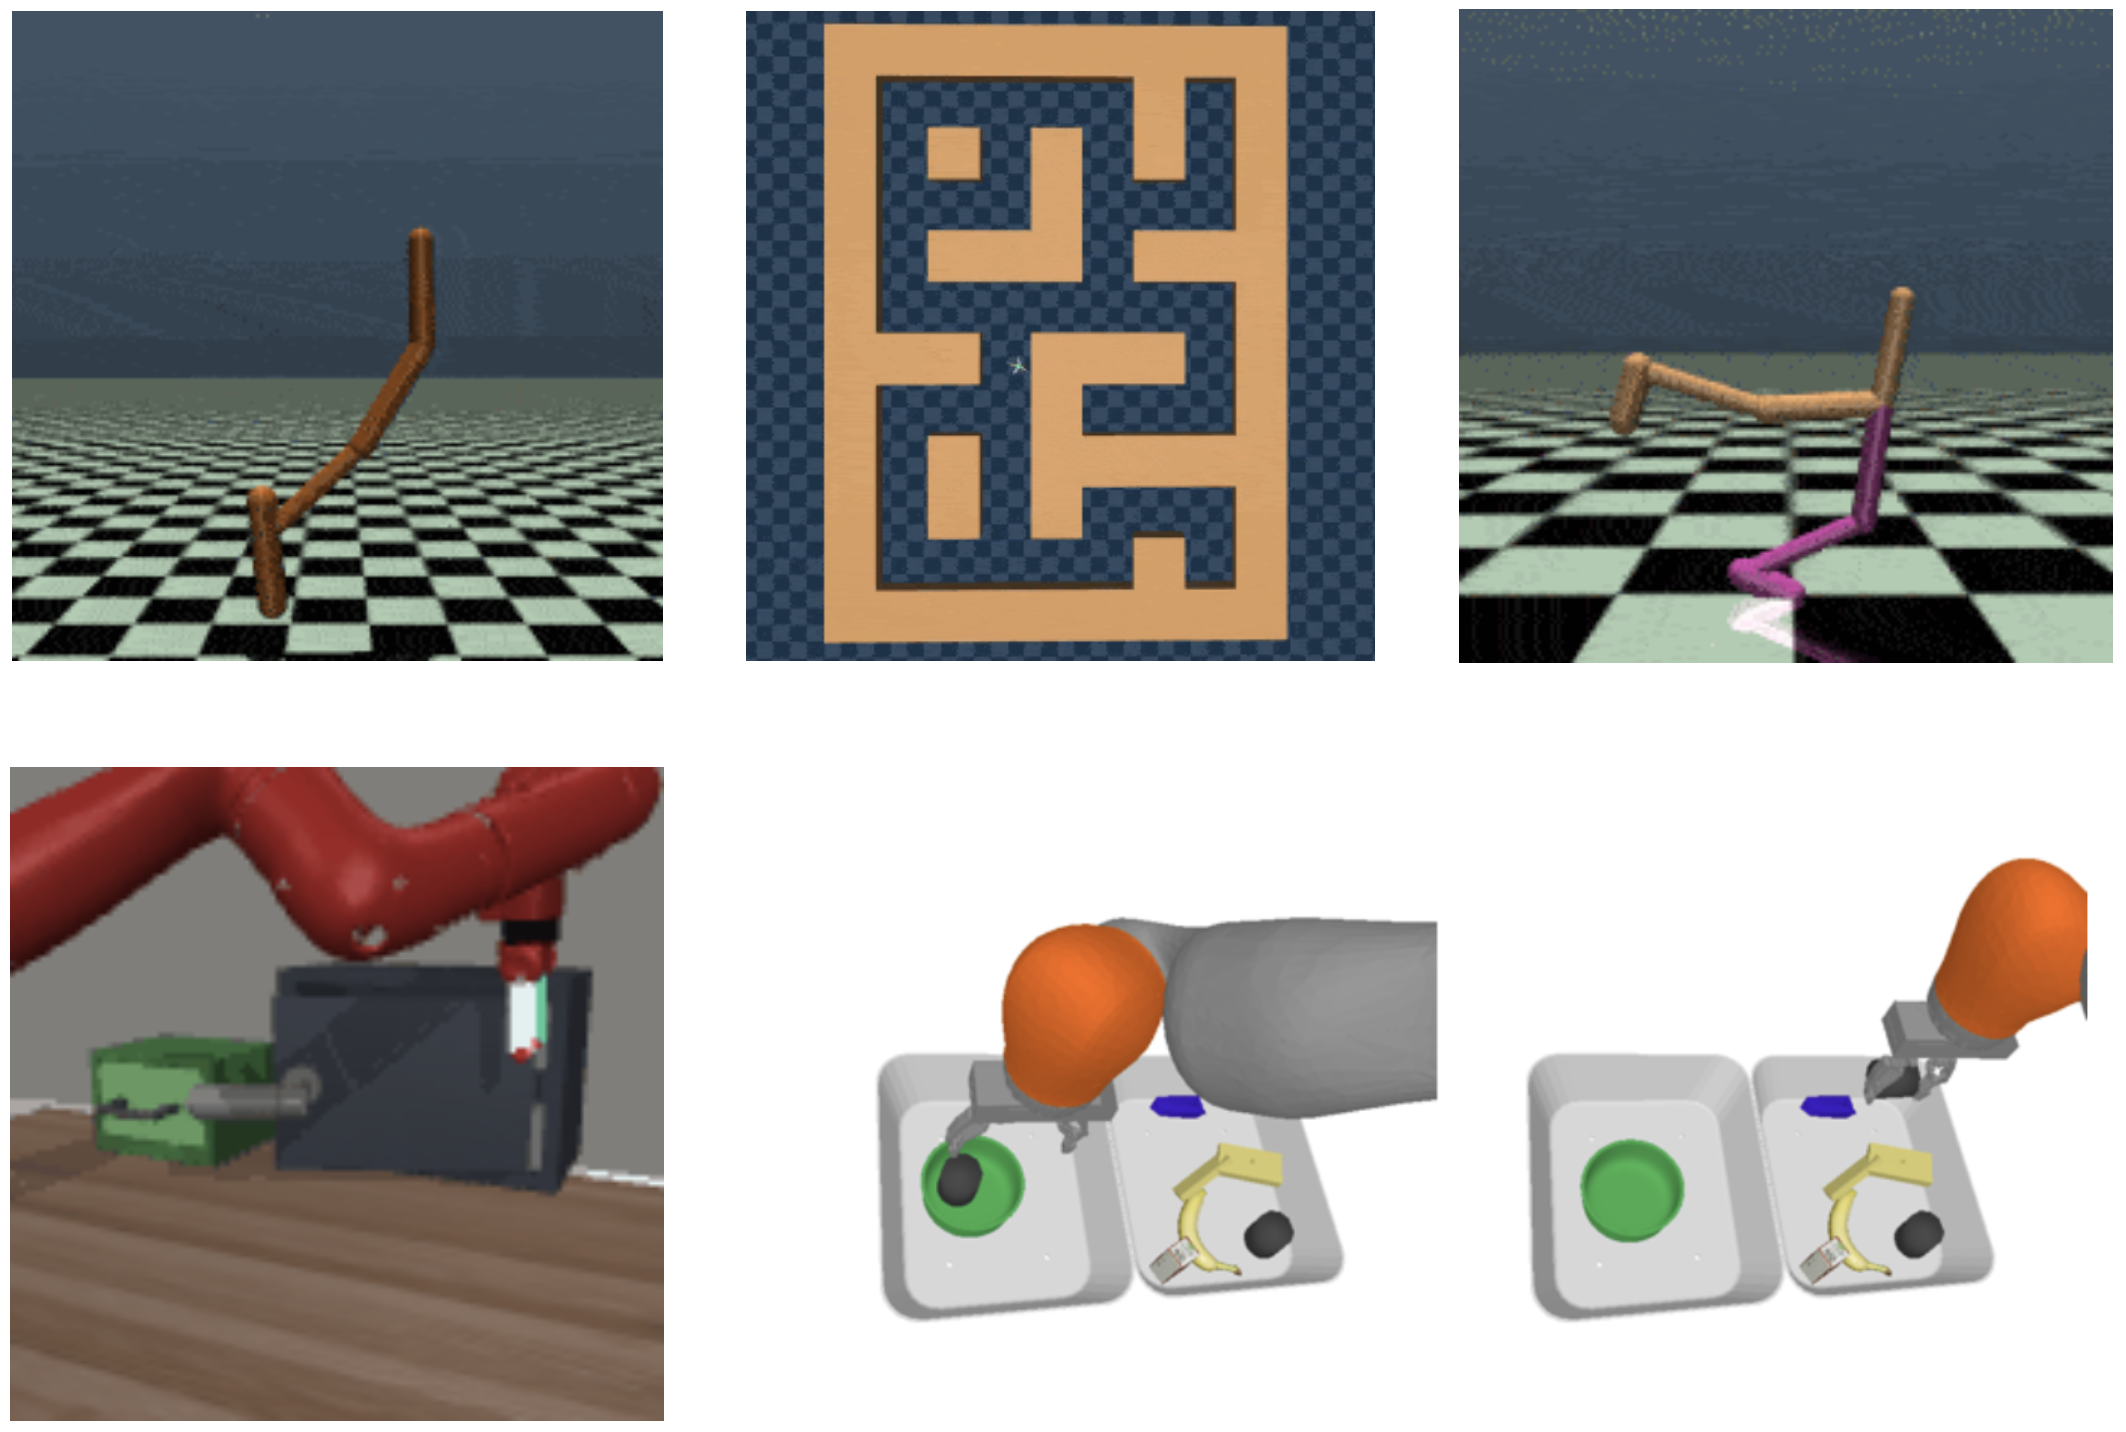
\includegraphics[width=0.35\textwidth]{chapters/uds/env.png}
    \vspace{-0.33cm}
    \caption{\footnotesize  Environments (from left to right):  single-task hopper, single-task and multi-task AntMaze, multi-task walker, multi-task Meta-World, and multi-task vision-based pick-place tasks.}
    \vspace{-0.35cm}
    \label{fig:env}
\end{figure}

\noindent \textbf{Single-task domains \& datasets.} We adopt two environments: hopper and the AntMaze from the D4RL benchmark~\citep{fu2020d4rl} for evaluation in the single-task setting. For the hopper environment, we consider two scenarios where we have 10k labeled data from the {hopper-expert} and 1M unlabeled transitions from the {hopper-random} datasets and {hopper-medium} datasets respectively. This setup is resembles practical problems where unlabeled data is of low-quality and even, irrelevant to the target task. For AntMaze, following the setup in \cite{yang2021trail}, we use 10k expert transitions as the labeled data and the entire datasets of {large-play} and {medium-play} as the unlabeled data.


\begin{table*}[ht]
\vspace{-0.3cm}
\caption{\footnotesize We perform an empirical analysis on the single-task environment \texttt{hopper} from D4RL~\citep{fu2020d4rl} benchmark to test the sensitivity of UDS under the data quality and data coverage for both the labeled task data and unlabeled data. The numbers are averaged over \final{ten} random seeds. We bold the best method without true reward relabeling. UDS outperforms No Sharing in 5 out of 6 settings while achieving competitive performances compared to Sharing All in 5 out of 6 settings.
CDS+UDS is able to further improve over UDS significantly in such a setting and also outperforms UDS in 5 out of 6 settings in general.
}
\vspace{-0.3cm}
\begin{center}
\resizebox{\textwidth}{!}{\begin{tabular}{l|l|l|rrr|rr}
\toprule
& & & & & & \multicolumn{2}{c}{\textbf{Oracle Methods}} \\
 \textbf{Environment} & \textbf{Labeled data type / size} & \textbf{Unlabeled data type / size}   & \textbf{CDS+UDS}   & \textbf{UDS}         & \textbf{No Sharing} & \textbf{CDS} & \textbf{Sharing All} \\
 \midrule
& \textbf{(a)} expert / 10k transitions & random / 1M transitions & \textbf{82.1}  & 78.8 & 77.1 & 83.3 & 86.1\\
& \textbf{(b)} expert / 10k transitions & medium / 1M transitions   & \textbf{78.1} & 64.8 & 77.1 & 82.5 & 64.6\\
& \textbf{(c)} expert / 10k transitions & expert / 990k transitions   & 106.1 & \textbf{108.4} & 77.1 & 106.6 & 112.3\\
 D4RL hopper  & \textbf{(d)} medium / 10k transitions & random / 1M transitions & \textbf{33.2}  & 9.9 & 28.7 & 41.2 & 38.9\\
& \textbf{(e)} medium / 10k transitions & expert / 1M transitions & \textbf{108.9}   & 106.7 & 28.7 & 111.1 & 107.5\\
& \textbf{(f)} random / 10k transitions & medium / 1M transitions & \textbf{63.5}  & 47.1 & 9.6 & 92.3 & 69.8\\
& \textbf{(g)} random / 10k transitions & expert / 1M transitions  & \textbf{101.2} & 95.9 & 9.6 & 110.9 & 102.8\\
\bottomrule
\end{tabular}}
\end{center}
\vspace{-0.7cm}
\label{tbl:single_task_analysis}
\normalsize
\end{table*}

\noindent \textbf{Multi-task domains \& datasets.} We consider several multi-task domains. The first set of domains are from prior work~\citep{yu2021conservative}: \textbf{(i)} the Meta-World~\citep{yu2020meta} domain, which consists of four tasks of opening and closing doors and drawers; and \textbf{(ii)} the Antmaze~\citep{fu2020d4rl} domain, which consists of mazes of two sizes (medium and large) with 3 and 7 tasks corresponding to different goal positions respectively. We also evaluate on the multi-task walker environment with dense rewards, which we will discuss in detail in Appendix~\ref{app:dense_reward}.
In addition, we test multi-task offline RL methods with UDS in the multi-task visual manipulation domain, which provides a realistic scenario, of the sorts we will encounter in robotic settings in practice. In this domain, there are 10 tasks with different combinations of object-oriented grasping, with 7 objects (banana, bottle, sausage, milk box, food box, can and carrot), as well as placing the picked objects onto one of three fixtures (bowl, plate and divider plate). For domains except the walker environment, we use binary rewards, where $1$ denotes the successful completion of the task and $0$ corresponds to failure. We also use the datasets used in \cite{yu2021conservative} for all domains. For details, see Appendix~\ref{app:env_data_details}.


\vspace{-0.1cm}
\subsubsection{Results of Empirical Evaluations}
\label{sec:results}
\vspace{-0.1cm}
\noindent \textbf{Results of Question (1) and (2).} We evaluate each method on the single-task hopper and AntMaze domains. As shown in Table~\ref{tbl:single_task}, we find that UDS outperforms No Sharing in 3 out of the 4 settings and reward learning methods in all the settings. We hypothesize that reward learning methods underperform because reward predictors are unable to achieve reasonable generalization ability in the limited labeled data setting. Note that UDS even achieves competitive performance as the oracle Sharing All method. Furthermore, an optimized reweighting scheme, i.e., CDS+UDS, is able to improve over UDS in each case, including cases where UDS fails to improve over No Sharing, indicating a large reward bias. These results testify to the effectiveness of optimizing for reweighting when dealing with unlabeled data. Note that on the AntMaze domain, CDS+UDS performs comparably to the recent approach~\citep{yang2021trail} that performs representation learning on the offline dataset first and then run offline training leveraging the learned representation. CDS+UDS also outperforms all the prior methods in offline training with learned representations discussed in \cite{yang2021trail}.

\noindent \textbf{Results of Question (3).} Observe in Table~\ref{tbl:gym} that UDS outperforms na\"ive multi-task offline RL without data sharing and reward learning methods, suggesting that leveraging unlabeled data with our simple method UDS can boost offline RL performance in both multi-task manipulation and navigation domains.
Since reward learning approaches obtain similar or worse results compared to No Sharing, which we suspect could be due to erroneous predictions on unseen transitions in the multi-task data, we only compare our methods to No Sharing and the oracle methods in the image-based experiments. As shown in Table~\ref{tbl:mtopt}, UDS outperforms No Sharing in 7 out of 10 tasks as well as the average task performance by a significant margin. Therefore, UDS is able to effectively leverage unlabeled data from other tasks and achieves potentially surprisingly strong results compared to more sophisticated methods that handle unlabeled offline data. We also find that CDS+UDS further improves upon the performance of UDS, which indicates that optimizing for reweighting via CDS+UDS can actually work well.




Finally, note that, CDS+UDS and UDS attain performance competitive with their oracle counterparts, CDS and Sharing All, that assume access to full reward information, both in Tables~\ref{tbl:gym} \& \ref{tbl:mtopt}. This is potentially very surprising, and one could hypothesize that this might be because most transitions in the unlabeled dataset were actually failures, and hence, were labeled correctly by UDS. However, to the contrary, our diagnostic analysis in Table~\ref{tbl:data_quality}, Appendix~\ref{app:data_quality} reveals that the unlabeled data \emph{does not} consist entirely of failures; in fact, around 60\% of the unlabeled data succeeds at the task of interest, indicating that the rewards are wrong for more than half the unlabeled data. In spite of this, UDS and CDS+UDS perform well. This indicates that UDS can be effective in removing the dependence of functional form of reward functions, which is often costly, without much loss in the performance and CDS+UDS can boost performance by reducing the bias.


\subsection{Empirical Analysis of UDS and CDS+UDS}
\label{sec:empirical_analysis}

To answer question (4), we analyze UDS and CDS+UDS on several offline RL problems designed to test robustness and sensitivity to the data coverage and the data quality on the single-task hopper domain. To create these instances, we consider 7 different combinations of data quality ({hopper-expert}, {hopper-medium} or {hopper-random}) and amount of labeled and unlabeled data labeled as \textbf{(a)}-\textbf{(g)} in Table~\ref{tbl:single_task_analysis}. In Appendix~\ref{app:mw_analysis}, we present results for a similar analysis in the multi-task Meta-World setting. We evaluate UDS, CDS+UDS and No Sharing in each case, and also present results for CDS and Sharing All approaches which assume access to the actual reward, for understanding. \final{Additionally, we conduct an ablation that compares UDS and CDS+UDS to reward learning methods in settings where the labeled data size and quality are varied, which is included in Appendix~\ref{app:reward_learning_ablation}.}


When the labeled data is of expert-level, adding unlabeled random or medium data (cases \textbf{a} and \textbf{b} in Table~\ref{tbl:single_task_analysis}) should only increase coverage, since the labeled data only consists of expert transitions. Moreover, the reward bias induced due to incorrect labeling of rewards on the medium unlabeled data should not hurt, since the 10k expert transitions retain their correct labels, and the medium/random data should only serve as negatives, provided the annotated rewards on this data are worse than the rewards in the expert data. Therefore, we expect the benefits of coverage to outweigh any reward bias; as seen in Table~\ref{tbl:single_task_analysis}, we find that UDS indeed helps compared to No Sharing. In particular, in those two cases, UDS approaches the oracle Sharing All method. 

Since reward bias is exacerbated when the unlabeled data is of higher quality and present in large amounts (cases \textbf{e, f, g}), it is reasonable to surmise that UDS will perform worse in such scenarios. However, on the contrary, in settings: random labeled data with medium or expert unlabeled data and medium labeled data with expert unlabeled data, we find that even though the rewards on the unlabeled transitions are incorrect, the addition of unlabeled data into training improves performance. This is because a higher quality unlabeled data improves the performance of the effective behavior policy, thereby improving performance for a conservative offline RL method. This result validates Theorem~\ref{prop:uds_ours}. 
We also conduct an ablation that varies the amount of unlabeled data in Appendix~\ref{app:unlabeled_dataset_size_analysis}. This ablation shows that the benefit of UDS reduces as the we reduce the amount of unlabeled data, which confirms our theory.

In the case where labeled data is medium and unlabeled data is random (case \textbf{d}), we find that UDS hurts compared to No Sharing. This is because the labeled data as well as unlabeled data are both low-medium quality and medium data already provides decent coverage (not as high as random data, but not as low as expert data). Therefore, in this case, we believe that the addition of unlabeled data neither provides trajectories of good quality that can help improve performance, nor does it significantly improve coverage, and only hurts by incurring reward bias. We therefore believe that UDS may not help in such cases where the coverage does not improve, and added data is not so high quality, which also agrees with our theoretical analysis. Furthermore, in the case where the labeled and unlabeled data are both expert (case \textbf{c}), UDS performs close to oracle methods CDS and Sharing All, which confirms the insights derived from Section~\ref{sec:uds_theory} that UDS does not introduce bias when the labeled and unlabeled data have the same distribution and hence should perform well.

Finally, note that CDS+UDS is able to improve over UDS in 5 out of 6 settings in hopper, suggesting that CDS+UDS gains benefit from reducing the reward bias as well as the sampling error shown in Section~\ref{sec:method}.



